\documentclass{beamer}
% Use jpg graphics in figure environments and pdflatex to compile!!!
\usepackage{graphicx,color,amsmath,amssymb,amsfonts,amsbsy,amsthm}
\usepackage{verbatim}
\usetheme{Berlin}
\newcommand{\includes}{/home/1104070/latex_include}
\newcommand{\dayonesegone}{day1_seg1_heuristic}
% Node the following tag will orient things right using dvi2pdf.
% Process with LaTeX first, then dvi2pdf.
\special{landscape}
% Fuzz -----------------------------------------------------------
\hfuzz5pt % Don't bother to report overfull boxes < 5pt
% MATH -----------------------------------------------------------
\input{\includes/kalman_cmdmaster.tex}
% THEOREM ENV. ---------------------------------------------------
\newtheorem{thm}{Theorem.}
\newtheorem{cor}[thm]{Corollary.}
\newtheorem{con}[thm]{Conjecture.}
\newtheorem{lem}[thm]{Lemma.}
\newtheorem{prop}[thm]{Proposition.}
\newtheorem{defn}[thm]{Definition.}
\renewcommand{\thethm}{}  % unnumbered
\pagestyle{plain}
%%% --------------------------------------------------------------
\newcounter{exercisecounter}
\begin{document}
\title{
\vfill \hrulefill \vfill
\begin{center}
Overview of Kalman Filter Theory and Navigation Applications\\
Day 1\\
Supplement
\end{center}
}
\author{Michael L. Carroll}
\date{Feb 24, 2004\\
\vfill \hrulefill \vspace*{.25in} \vfill
\begin{tiny}
\copyright 2003 by Michael L. Carroll
\end{tiny}
} \maketitle
% ----------------------------------------------------------------
\begin{frame}
\textbf{Day 1: The Basic Kalman Equations, Part I\\
Segments}
 \begin{itemize}
 \item Ionospheric Probe (Gelb)
 \item Baro-Inertial Vertical Channel
 \item Simulink Example Geogrphic Position Rate Equations
\end{itemize}
\end{frame}

\begin{frame}
Ionospheric Probe
\begin{itemize}
  \item Balloon Launched Ionosphereic Probe
  \item Example originally due to Gelb
  \item Grewal and Andrews have also presented it
  \item Illustrates single-axis, short-term inertial error dynamics
\end{itemize} 
\end{frame}

\begin{frame}
Ionosphereic Probe: Continuous Model
\begin{equation}\label{ionoprobemodel}
\delta p(t)\approx \delta p(0) + \delta v(0) t + \delta a(0) \frac{t^2}{2}
\end{equation} 
where $\delta p=INS $position error, $\delta v=$velocity error, $\delta a=$acceleration error.

Assume $\delta \dot{a}=0$.

State model: $x_1(t) = \delta p(t)$, $x_2(t)=\dot{x}_1(t)$, $x_3(t)=\dot{x}_2(t)$
\end{frame}

\begin{frame}
Ionospheric Probe: Model $\dot{x}=Fx$

State Dynamics Model (with companion matrix):
\begin{equation}
\begin{bmatrix}
\dot{x}_1\\
\dot{x}_2\\
\dot{x}_3
\end{bmatrix}
=
\begin{bmatrix}
0 &1 &0\\
0 &0 &1\\
0 &0 &0
\end{bmatrix}
\begin{bmatrix}
x_1\\
x_2\\
x_3
\end{bmatrix}
\end{equation} 
or
\[
\begin{bmatrix}
\delta\dot{p}\\
\delta\dot{v}\\
\delta\dot{a}
\end{bmatrix}
=
\begin{bmatrix}
0 &1 &0\\
0 &0 &1\\
0 &0 &0
\end{bmatrix}
\begin{bmatrix}
\delta p\\
\delta v\\
\delta a
\end{bmatrix}
\]
\end{frame}

\begin{frame}
State Transistion Matrix $\Phi(t)$

As matrix exponential $\Phi(t)=\exp{Ft}=e^{Ft}$

\begin{equation}
\Phi(t)=e^{Ft}= I + Ft + \dfrac{F^2t^2}{2!}+ \dfrac{F^3t^3}{3!}+\cdots=
\begin{bmatrix}
1 &t &\dfrac{t^2}{2}\\
0 &1 &t\\
0 &0 &1
\end{bmatrix}
\end{equation}
because $F^n=0$ for all $n\geq 3$.

Note also that here $\Delta t= t-0=t$ in this example. 
\end{frame}

\begin{frame}
Ionospheric Probe: Measurement Model
\begin{itemize}
\item Radio-indicated position and INS indicated position.
\item Scalar measurement formed by differencing the two indicated positions
\end{itemize}
\begin{align*}
z &= p_{\text{radio}} - p_{\text{INS}}\\
  &= (p_{\text{true}}+\delta p_{\text{radio}}) -
(p_{\text{true}}+\delta p)\\
  &=-\delta p + \delta p_{\text{radio}}
\end{align*}
Thus, $H=\begin{bmatrix}-1&0&0\end{bmatrix}$ and measurement noise $v=\delta p_{\text{radio}}$
\end{frame}

\begin{frame}
Exercise:  Solve the discrete Kalman equations for $K_k$, $P_k(+)$ and $\hat{x}_k(+)$ using

$t_0=0.0$, $t_1=0.5$, $t_2=1.0$

The equations to solve are:
\[\kalgaineq\]
\[\covupdateeq\]
\[\stateupdateeq\]
Assume $\hat{x}_0(+)=0$, $P_0(+)=\begin{bmatrix}
p_{11}(0)&0&0\\
0&p_{22}(0)&0\\
0&0&p_{33}(0)
\end{bmatrix}$
with $p_{11}(0)=(1 \text{nm})^2$, $p_{22}(0)=(7.3 \text{kts})^2$, $p_{33}(0)\neq 0$.  Also, assume measurement noise standard deviation is $\sigma_{\text{radio}}= 30 \text{ft}$
\end{frame}

\begin{frame}
Ionospheric Probe: Solution Approach
\begin{itemize}
  \item First extrapolate $\hat{x}_0(+)$ to time $t_1=30$ sec using $\Phi(30)$ to get $\hat{x}_1(-)$
  \item Extrapolate $P_0(+)$ to get $P_1(-)$ using $\Phi(30)$ and $\Phi\trans(30)$.  There is no process noise in this problem.
  \item Compute Kalman gain at $t_1=30$
  \item Update the state estimate and the error covariance.
\end{itemize} 
\end{frame}

\begin{frame}
Baro-Inertial Vertical Channel
\begin{itemize}
  \item Plumb-Bob Gravity and Gravity Modeling
  \item Vertical Channel
\end{itemize} 
\end{frame}

\begin{frame}
Plumb-Bob Gravity
\begin{itemize}
  \item Gravitational acceleration as would be sensed by a plumb-bob: true gravity plus centripetal force
  \item Changes with location and altitude
  \item Very closely aligned with geodetic vertical
  \begin{itemize}
    \item geodetic vertical: normal to ellipsoid
  \end{itemize} 
\end{itemize} 
\[g'=g-\eratevec\times(\eratevec\times r)\]
\end{frame}

\begin{frame}
Plumb-Bob Gravity
\begin{itemize}
  \item Horizontal components $\approx$ 0 at earth's surface in local level coordinate frame
  \item Altitude dependent term can be added 
\end{itemize} 
\end{frame}


\begin{frame}
Gravity Model

\begin{eqnarray}
 g'&= G_1 - 2G_1(\dfrac{h}{R_e} - e \sin^2\lat  )\\
& +\dfrac{3}{2}J_2G_1(1-3\sin^2\lat)\nonumber\\
& \;\;\;\;\;\;\;\;\;\;\;\;\;\;\;\;\; - R_e\norm{\eratevec}^2(1-e\sin^2\lat+\dfrac{h}{R_e})\cos^2\lat \nonumber
\end{eqnarray}
% \[ g'= G_1(1-2\dfrac{h}{R_e}+2e \sin^2\lat) +\dfrac{3}{2}J_2G_1(1-3\sin^2\lat)-R_e\norm{\eratevec}^2(1-e\sin^2\lat\dfrac{h}{R_e})\cos^2\lat\]
where
\begin{tiny}
\begin{align*}
g' &= \text{plumb-bob gravity magnitude}\\
G_1&= \text{mean gravity magnitude at earth's surface on equator}\\
h  &= \text{altitude}\\
R_e&= \text{mean earth equatorial radius}\\
e  &= \text{earth's ellipticity 1/298}\\
\lat&= \text{geodetic latitude}\\
J_2&= \text{empirical constant}=0.00108\\
\eratevec&= \text{earth rate vector}
\end{align*}
\end{tiny}
\end{frame}


\begin{frame}
Baro-Inertial Vertical Channel 
\begin{itemize}
  \item Inertial errors and gravity model inaccuracies conspire to make the vertical channel unstable
  \begin{itemize}
	\item Integrated outputs of Z accelerometer yield altitude errors
    \item But the gravity model is a function of altitude!
	\item Vicious circle: erroneous gravity enters into integration of vertical acceleration
  \end{itemize}
\end{itemize} 
\end{frame}

\begin{frame}
Baro-Inertial Vertical Channel
\begin{itemize}
  \item Stabilize loop by using difference between barometric altitude and INS-indicated altitude
  \item Baro altitude has long-term stability
  \item INS altitude has wide bandwidth, i.e., responds well to sudden changes in altitude
  \item Difference between baro and inertial altitude is used as a feedback signal
\end{itemize} 
\end{frame}
\begin{frame}
\begin{center}
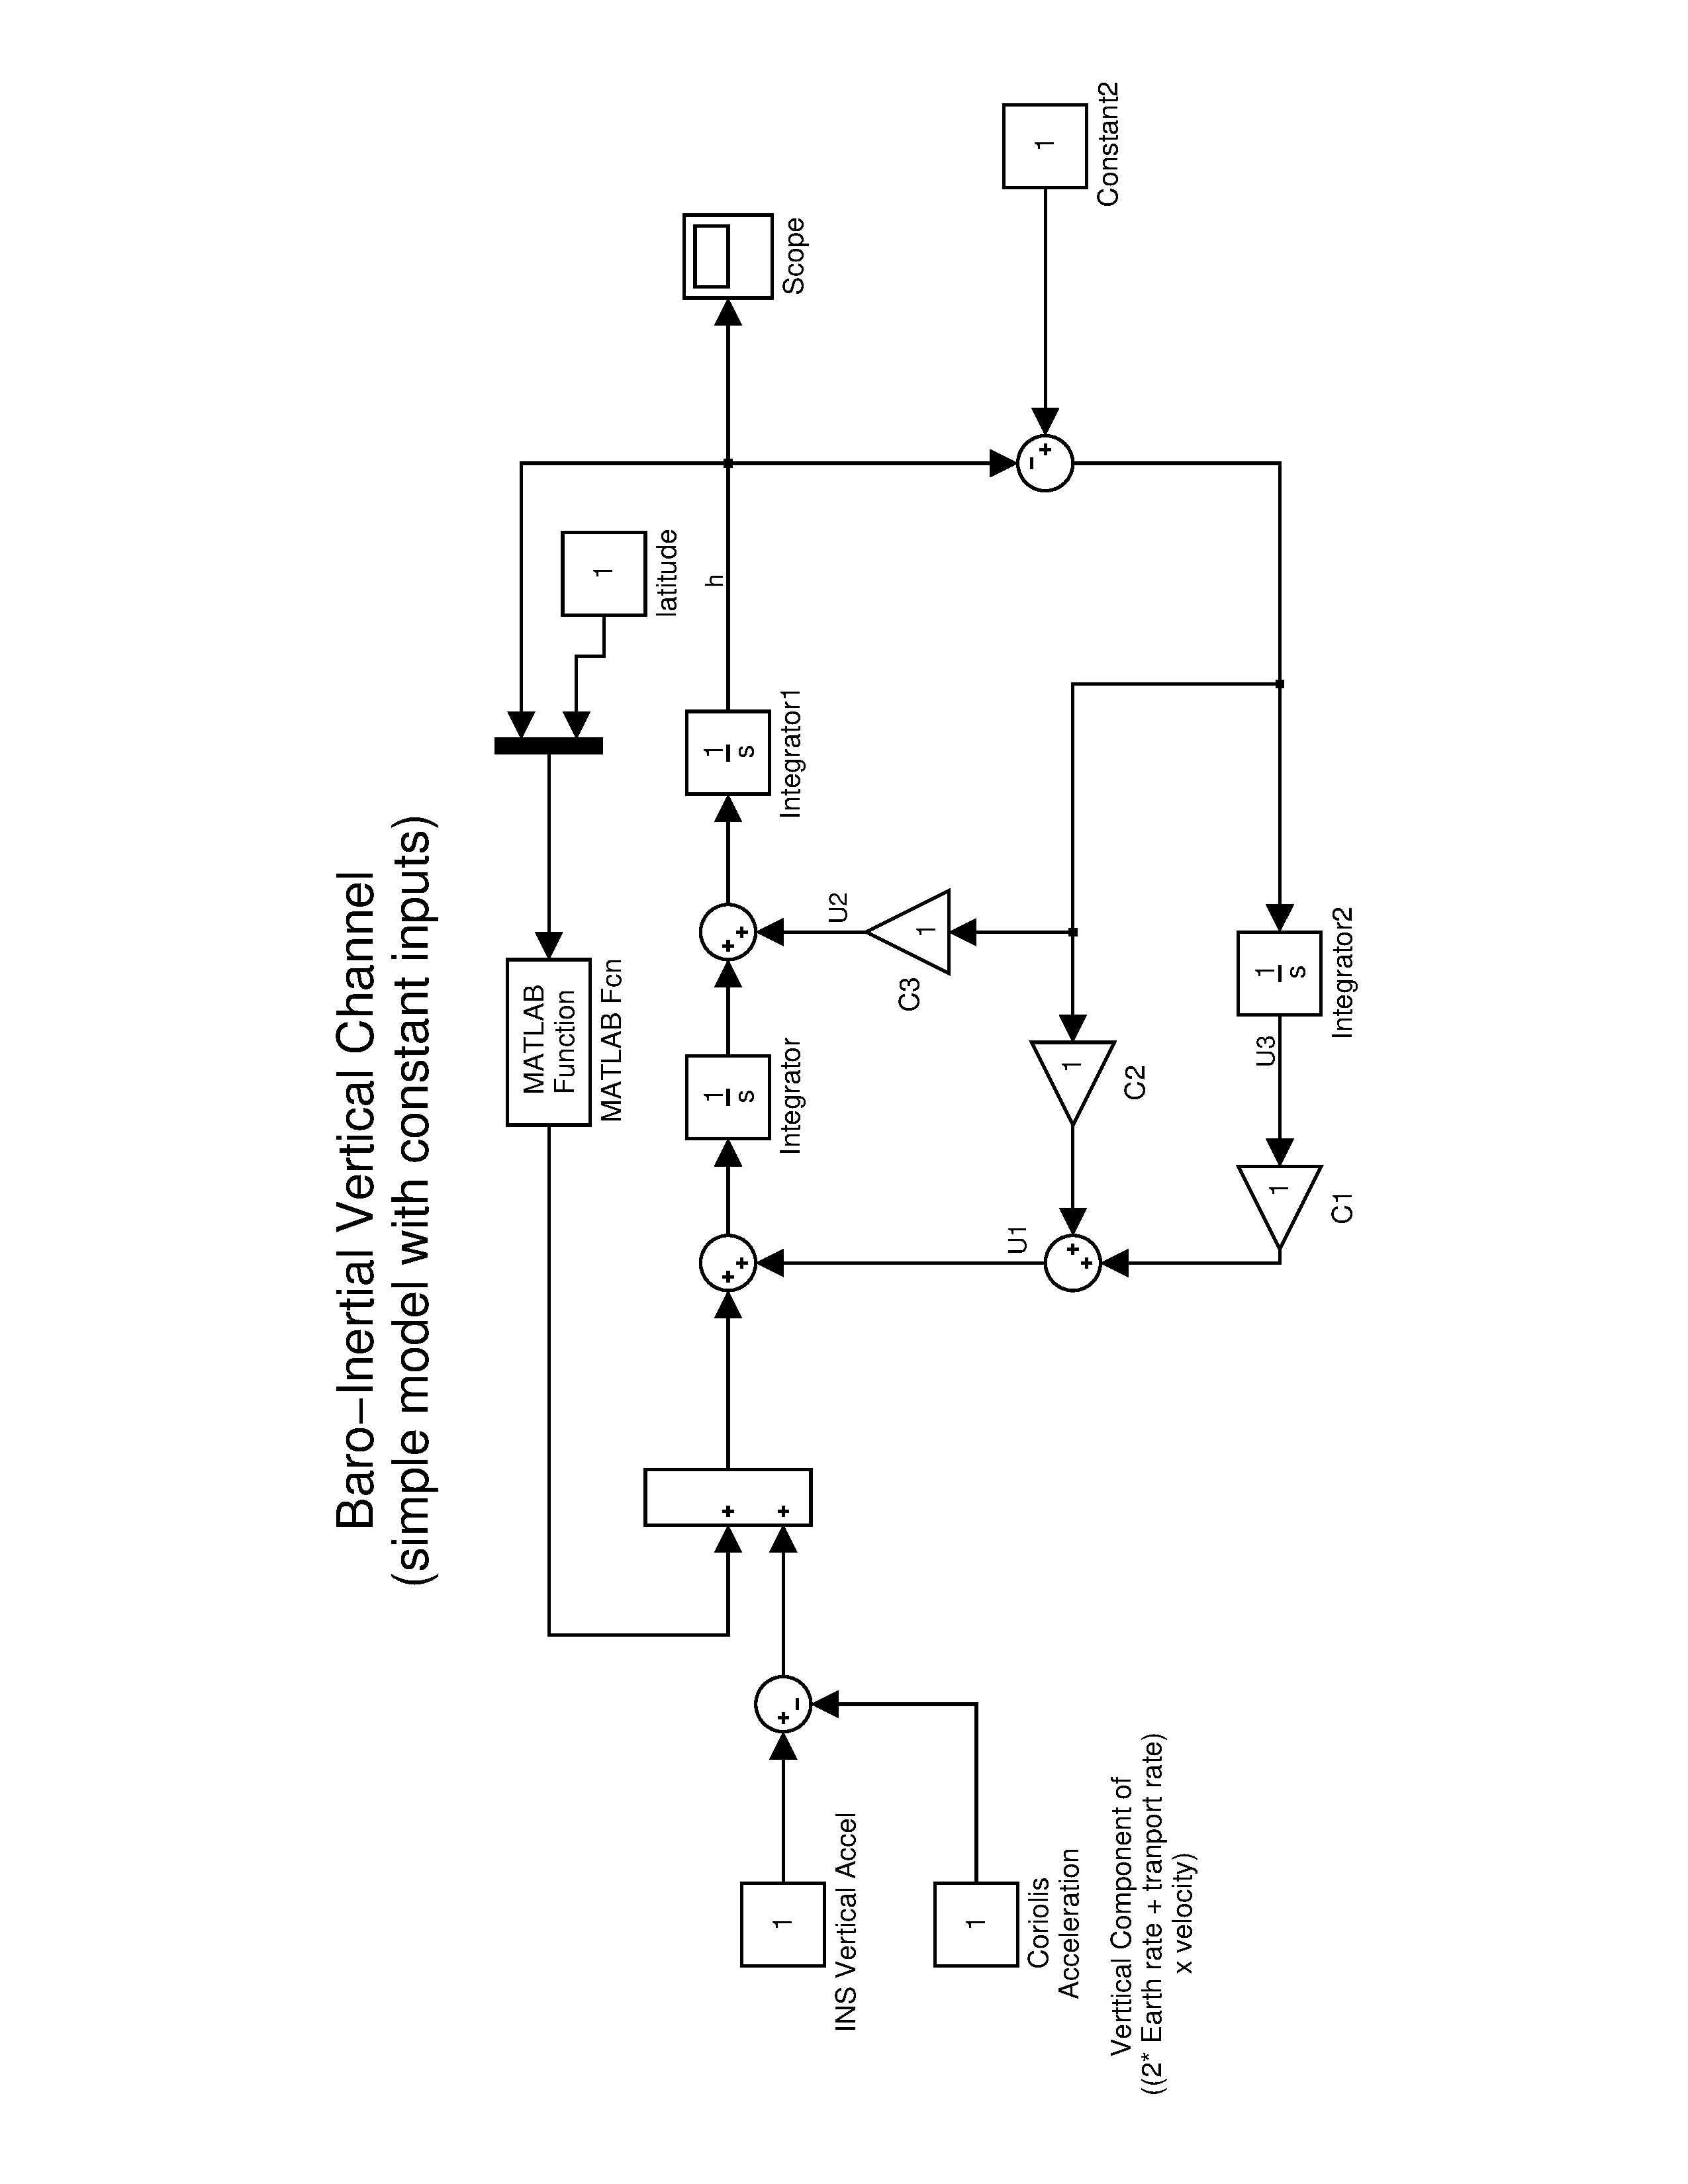
\includegraphics[angle=-90,width=\textwidth]{matlab/baro_inertial.jpg}
\end{center}
\end{frame}
% ----------------------------------------------------------------
\end{document}
